\documentclass[11pt]{article}

\usepackage[a4paper,margin=1in]{geometry}
\usepackage{amsmath,amssymb}
\usepackage{graphicx}
\usepackage{booktabs}
\usepackage{array}
\usepackage{enumitem}
\usepackage{microtype}
\usepackage{lineno}
\usepackage{caption}
\usepackage[colorlinks=true,linkcolor=black,citecolor=black,urlcolor=black]{hyperref}

\setlength{\parindent}{0pt}
\setlength{\parskip}{0.68em}
\setlist[itemize]{leftmargin=1.35em,itemsep=0.20em,topsep=0.20em}
\setlist[enumerate]{leftmargin=1.35em,itemsep=0.20em,topsep=0.20em}
\linenumbers

\newcommand{\E}{\mathbb{E}}
\newcommand{\Var}{\operatorname{Var}}
\newcommand{\tr}{\operatorname{tr}}
\newcommand{\X}{\mathcal{X}}
\newcommand{\Aint}{\mathcal{A}^{I}}
\newcommand{\Schan}{\mathcal{S}^{I}}
\newcommand{\DeltaStrong}{\Delta_{\mathrm{strong}}}
\newcommand{\ANK}{\mathcal{A}^{NK}}
\newcommand{\PNK}{P^{NK}}
% Automatically generated by nk_channel_simulation.py
\newcommand{\NKDeltaSmooth}{0.004}
\newcommand{\NKDeltaIntermediate}{0.018}
\newcommand{\NKDeltaHighBroad}{-0.085}
\newcommand{\NKPositiveIntermediate}{0.56}
\newcommand{\NKBadNaiveHighBroad}{0.49}
\newcommand{\NKBadChannelHighBroad}{0.49}

% Automatically generated by nk_local_channel_index.py
\newcommand{\NKChannelRtwoBaselineHFive}{0.294}
\newcommand{\NKChannelRtwoIndexHFive}{0.438}
\newcommand{\NKChannelRtwoPlusHFive}{0.517}
\newcommand{\NKChannelRtwoGainHFive}{0.144}
\newcommand{\NKChannelRtwoFullGainHFive}{0.223}
\newcommand{\NKChannelCoefIndexHFive}{0.0213}
\newcommand{\NKChannelLowBinGainHFive}{-0.0019}
\newcommand{\NKChannelHighBinGainHFive}{0.0888}
\newcommand{\NKChannelHighLowDiffHFive}{0.0908}
\newcommand{\NKChannelCorrHFive}{0.608}

% Automatically generated by nk_robustness_checks.py
\newcommand{\NKRobustMinIndexGain}{0.063}
\newcommand{\NKRobustMaxIndexGain}{0.133}
\newcommand{\NKRobustMinChannelGain}{0.134}
\newcommand{\NKRobustMaxChannelGain}{0.234}
\newcommand{\NKRobustMeanCorr}{0.538}


\title{\vspace{-1.5cm}\textbf{Interactional intelligence as an evolutionary channel}}
\author{Daniel Ortiz-Barrientos$^{1,*}$}
\date{\vspace{-0.5em}\small $^1$School of the Environment, The University of Queensland, Brisbane, Australia.\\
$^*$Correspondence: d.ortizbarrientos@uq.edu.au\\[0.6em]
\textit{Draft v0.5. Author list, funding and acknowledgements to be finalised.}}

\begin{document}
\maketitle

\begin{abstract}
\noindent Intelligence is usually assigned to individual minds or to machines. We propose a different unit of analysis: the coupled human--AI system moving through an epistemic landscape. Interactional intelligence emerges when such a system generates, evaluates and stabilises useful movement better than either component alone. We formalise this claim as a channel theory. A proposal operator describes the directions of change the coupled system can generate; an evaluative gradient describes local improvement; landscape curvature describes the risk that plausible steps fail when combined or extended. A minimal NK model shows that complementarity is conditional, not automatic, and that a local channel index predicts realised improvement over subsequent search steps. The theory yields testable predictions for branching conversations, memory structures, role partitioning and multi-agent systems. It does not infer machine consciousness from performance. It makes the intelligence of coupled cognitive systems measurable.
\end{abstract}

\textbf{Central claim.} Interactional intelligence emerges when a coupled human--AI system generates, evaluates and stabilises useful movement through an epistemic landscape better than either component alone.

\section*{A misplaced unit}

Public debate about artificial intelligence often asks whether a machine will exceed human intelligence. That question has value, but it can misidentify the cognitive unit that matters in scientific work. Many problems are not solved by a brain alone or by a machine alone. They are solved by a loop: a human with goals and judgement, a model with generative capacity, an interface with constraints, a shared artefact that stores partial progress, and an environment that supplies feedback.

This view has intellectual ancestors. Extended-mind and distributed-cognition theories argued that cognition can be partly constituted by external artefacts, social procedures and representational systems \cite{Clark1998,Hutchins1995,Hollan2000}. Human--AI systems make that claim experimentally tractable. We can perturb the components of the loop, branch the history of a conversation, control memory and model access, and evaluate the resulting artefacts blind to condition.

The empirical literature already shows why this is needed. Human--AI combinations do not automatically outperform their parts. A recent meta-analysis found that human--AI combinations were, on average, worse than the best of human or AI alone, even though they often improved performance relative to humans alone \cite{Vaccaro2024}. Newer frameworks therefore define complementarity as the condition in which human--AI teams outperform either humans alone or AI systems alone, and treat this as a design and measurement problem rather than as a default property of AI use \cite{Gonzalez2026}. Field evidence from knowledge work also indicates a jagged frontier: AI can help on some tasks while hurting on nearby tasks that appear similar to users \cite{DellAcqua2026}.

We need a theory that explains this heterogeneity. The claim developed here is that intelligence in human--AI systems depends on the geometry of interaction. A coupled system succeeds when the variation it can generate is aligned with the directions that improve the artefact, and when the human, model and memory structure can detect and manage curvature in the task landscape. It fails when fluent proposals move in directions that the human cannot evaluate, when memory preserves the wrong state, or when local improvements combine badly.

\begin{figure}[t]
\centering
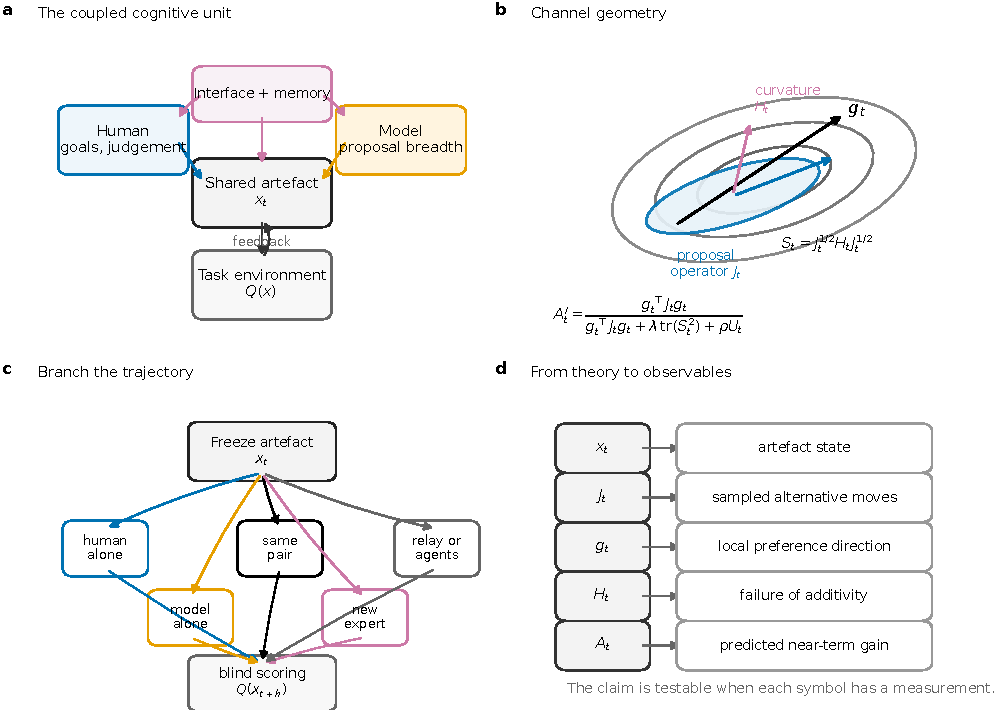
\includegraphics[width=0.97\linewidth]{figures/fig1_conceptual_framework.pdf}
\caption{\textbf{Interactional intelligence as a coupled channel.} \textbf{a}, The proposed cognitive unit is a loop containing a human, a model, an interface, memory, a shared artefact and a task environment. \textbf{b}, The channel theory separates the local evaluative gradient $g_t$, accessible proposal variation $J_t$, curvature $H_t$ and evaluator uncertainty. \textbf{c}, Branching experiments freeze an artefact and randomise continuation to isolate the contribution of the human, model, artefact and coupling regime. \textbf{d}, Each theoretical object has an empirical counterpart, making the analogy measurable rather than metaphorical.}
\label{fig:conceptual}
\end{figure}

\section*{A channel theory}

Let $x_t \in \X$ denote the state of an intellectual artefact at time $t$. The artefact could be a proof, model, paragraph, codebase, manuscript plan, simulation design or experimental protocol. Let
\begin{equation}
    Q: \X \rightarrow \mathbb{R}
\end{equation}
be a task-specific quality function. Higher values of $Q$ mean that the artefact is more correct, explanatory, useful, reproducible or fit for the purpose at hand. The function $Q$ need not be known exactly. It can be estimated by objective tests, blinded expert judgement, predictive performance, proof verification, code tests or combinations of these.

The phrase \emph{epistemic landscape} refers to this mapping from artefacts to quality. Around the current artefact, the local direction of improvement is
\begin{equation}
    g_t = \nabla Q(x_t),
\end{equation}
and the local curvature is
\begin{equation}
    H_t = \nabla^2 Q(x_t).
\end{equation}
The gradient tells us which small changes improve the artefact. The Hessian tells us how the value of those changes depends on context. A task with weak curvature is forgiving: useful small changes remain useful when combined. A task with strong curvature is less forgiving: two locally plausible changes can interact, cancel each other or break the argument.

A human--AI system does not search all possible artefacts. It samples a restricted set of changes shaped by the human's expertise, taste, attention, prompts and scepticism; by the model's training, context window and stochasticity; and by the interface and shared memory. We describe this accessible variation by a proposal distribution
\begin{equation}
    P_C(u \mid x_t),
\end{equation}
where $C$ denotes the coupling regime: human alone, model alone, ordinary chat, role-partitioned collaboration, persistent memory, agent relay or any other experimental condition. For local proposals, define the covariance operator
\begin{equation}
    J_t(C) = \E_C[u u^\top \mid x_t].
\end{equation}
This operator is the cognitive analogue of an additive genetic covariance matrix. In quantitative genetics, $G$ describes the directions of phenotypic change available to selection, and the breeder's equation maps a selection gradient into expected response,
\begin{equation}
    \Delta \bar z = G\beta.
\end{equation}
Here, $J_t$ describes the directions of intellectual change available to the coupled system.

The key local result is simple. Suppose proposals are initially symmetric around zero and that the system preferentially develops proposals according to their local value. For weak development intensity $\eta$, the weight on proposal $u$ is approximately proportional to
\begin{equation}
    \exp(\eta g_t^\top u).
\end{equation}
A first-order expansion gives
\begin{equation}
    \E_C[u \mid \text{developed},x_t] \approx \eta J_t(C) g_t. \label{eq:response}
\end{equation}
Thus the expected movement of the coupled system depends on the alignment between accessible variation and evaluative gradient. A system can sound intelligent while having a poor proposal operator. It can generate many words yet fail to move along $g_t$. Conversely, a system with modest generative breadth can make strong progress if its accessible variation is aligned with useful directions and if the human can select among proposals well.

Curvature enters through the second-order expansion
\begin{equation}
    Q(x_t+u)-Q(x_t) \approx g_t^\top u + \frac{1}{2}u^\top H_tu.
\end{equation}
The linear term measures directional progress. The quadratic term measures how the landscape bends along the proposed direction. When curvature is high in directions the system frequently samples, linear extrapolation becomes unreliable.

We therefore define the interactional channel operator
\begin{equation}
    \Schan_t = J_t^{1/2} H_t J_t^{1/2}. \label{eq:channel_operator}
\end{equation}
This operator expresses task curvature in the coordinates of accessible moves. A useful bounded channel index is
\begin{equation}
    \Aint_t =
    \frac{g_t^\top J_t g_t}
    {g_t^\top J_t g_t + \lambda\,\tr[(\Schan_t)^2] + \rho U_t},
    \label{eq:interactional_channel_index}
\end{equation}
where $U_t$ is evaluator uncertainty, and $\lambda$ and $\rho$ set the scale of curvature and uncertainty relative to linear signal. The numerator is useful movement available through the current coupling regime. The denominator adds the liabilities that make local extrapolation fail.

Strong complementarity is then
\begin{equation}
    \DeltaStrong(\tau)=
    \E[Q_{HM,\tau}]-\max\{\E[Q_{H,\tau}],\E[Q_{M,\tau}]\},
    \label{eq:strong_complementarity}
\end{equation}
for task class $\tau$. Interactional intelligence, in the operational sense used here, is sustained positive strong complementarity across tasks or across phases of the same task. Augmentation relative to the human alone is useful, but it is not yet strong complementarity.

The proposition is therefore: if a coupled system samples proposals from $J_t$, develops them according to an estimate of $g_t$, and stabilises them before transmission, then near-term progress is controlled by the alignment term $g_t^\top J_tg_t$ and by the curvature and uncertainty liabilities in Equation \ref{eq:interactional_channel_index}. This does not prove that any real human--AI system is intelligent. It states the conditions under which such a system should improve.

\section*{From metaphor to measurement}

The evolutionary analogy is useful only if it changes what we measure. It should not make us say that a conversation is literally natural selection, or that intelligence is a substance moving from a machine into a human. Its purpose is narrower: to separate variation, evaluation and transmission in a coupled cognitive system.

The first discipline is operator typing. Each verbal claim must correspond to a typed object. The artefact $x_t$ lives in an idea space $\X$. A proposal $u$ is a possible local change to that artefact. The quality function $Q$ defines improvement for the task. The gradient $g_t$ is the local direction of improvement; the proposal operator $J_t$ describes the directions the coupled system can generate; and the Hessian $H_t$ describes how those directions interact. In this language, ``more creativity'' means a change in accessible variation, ``better judgement'' means a better estimate of the evaluative gradient, and ``dangerous fluency'' means confident movement through directions where curvature is high.

The second discipline is logical separation. A theory of interactional intelligence must keep definitions, mechanisms and tests apart. The definition is strong complementarity. The proposed mechanism is channel alignment. The tests are branching conversations, local operator estimation, NK landscapes and agent systems. If a human--AI pair beats the human alone, that is augmentation; it is not yet strong complementarity. If the pair fails, the failure is not merely a negative result. It becomes diagnostic evidence about proposal quality, evaluation, memory, role partitioning or curvature.

The third discipline is combinatorial. The object of study is not a single transcript. It is the branching graph of possible continuations from a shared artefact. Nodes are artefact states; edges are moves that propose, evaluate, revise or stabilise a change. A realised conversation is one path through this graph. A branching experiment samples nearby paths under different coupling regimes: the same human, a new human, the model alone, a relay chain, an agent population or a compressed memory state. This is how the theory asks where the intelligence resides.

\begin{table}[t]
\centering
\small
\caption{\textbf{Measurement map for interactional intelligence.} The theory becomes testable when each mathematical object has an empirical estimator.}
\begin{tabular}{p{0.12\linewidth}p{0.32\linewidth}p{0.46\linewidth}}
\toprule
Object & Meaning & Empirical estimator \\
\midrule
$x_t$ & Current artefact state & Manuscript, proof, code, model, protocol or decision record at turn $t$ \\
$Q(x_t)$ & Task quality & Blinded expert score, code tests, proof validity, prediction error, reproducibility or weighted composite \\
$J_t$ & Accessible proposal variation & Sampled alternative next moves under controlled prompts, memory states or coupling regimes \\
$g_t$ & Local evaluative direction & Pairwise preference data, expert-ranked local edits, objective test improvements \\
$H_t$ & Curvature or interaction among moves & Failure of additivity when two or more local changes are combined \\
$U_t$ & Evaluator uncertainty & Disagreement among raters, noisy test outcomes, calibration error or model-version variability \\
$\Aint_t$ & Channel index & Useful local signal divided by signal plus curvature and uncertainty liability \\
\bottomrule
\end{tabular}
\label{tab:measurement_map}
\end{table}

\section*{A minimal NK test}

NK landscapes provide a first toy test because they separate two quantities that the theory says must not be confused: the breadth of accessible moves and the reliability of evaluation on a curved landscape \cite{Kauffman1987,Weinberger1991}. We used binary artefacts $x\in\{0,1\}^N$ with $N=16$. Quality was the mean of $N$ local contributions, each depending on one component and $K$ other components. Low $K$ gives a smoother epistemic landscape; high $K$ gives a more rugged landscape in which locally plausible moves interact.

We compared four search regimes. The human-like searcher ($H$) made few, mostly local proposals and evaluated them with relatively low noise. The model-like searcher ($M$) made more and broader proposals, with maximum Hamming distance $D$, but evaluated them with greater noise and a bias towards broad moves. A naive coupled system ($HM_{naive}$) combined human-like and model-like proposals, then accepted any move that appeared locally beneficial to the human-like evaluator. A stabilised coupled system ($HM_{channel}$) used the same proposals and evaluator, but accepted a move only when the estimated gain exceeded an uncertainty margin. This margin is a minimal representation of checking, role partitioning and memory compression.

For each pair of $K$ and $D$, we simulated 32 paired landscapes and starting states for 50 steps, using the same landscape and start for all four regimes. The relevant outcome was strong complementarity,
\begin{equation}
    \DeltaStrong = Q(HM_{channel}) - \max\{Q(H),Q(M)\}.
\end{equation}
A positive value means that the stabilised coupled system beat both solo components on the same landscape.

The result is qualitative rather than evidential, but it is informative. Smooth landscapes gave little strong complementarity: at $K=0$ and $D=4$, $\DeltaStrong=\NKDeltaSmooth$. In an intermediate landscape, coupled search did better: at $K=4$ and $D=4$, $\DeltaStrong=\NKDeltaIntermediate$, with positive strong complementarity in $\NKPositiveIntermediate$ of paired runs. Under high ruggedness and excessive proposal breadth, the channel failed: at $K=12$ and $D=8$, $\DeltaStrong=\NKDeltaHighBroad$. Thus proposal diversity was not intrinsically useful. It helped when evaluation and stabilisation could manage the curvature induced by $K$, and it hurt when broad moves exceeded that capacity.

The NK model also lets us test the local operator claim directly. At a state $x_t$, let $U$ be a sampled set of bit flips from the proposal distribution of the stabilised coupled system. The true quality change is
\begin{equation}
    \Delta_t(U)=Q(x_t \oplus U)-Q(x_t),
\end{equation}
where $\oplus$ denotes bitwise flipping. The local additive prediction is the sum of the single-bit effects available at the same state,
\begin{equation}
    L_t(U)=\sum_{i\in U} \{Q(x_t \oplus i)-Q(x_t)\},
\end{equation}
and the nonlinear residual is
\begin{equation}
    R_t(U)=\Delta_t(U)-L_t(U).
\end{equation}
This decomposition is the finite-state analogue of separating a linear channel from curvature.

For the proposal distribution $\pi_t(U)$, define the local NK channel index
\begin{equation}
    \ANK_t =
    \frac{\E_{\pi_t}[(L_t(U)_+)^2]}
    {\E_{\pi_t}[(L_t(U)_+)^2]+\E_{\pi_t}[R_t(U)^2]+\E_{\pi_t}[\sigma_t(U)^2]},
    \label{eq:nk_local_channel}
\end{equation}
where $L_+=\max(L,0)$ and $\sigma_t(U)^2$ is the evaluator's uncertainty for a proposal of that size. This index is high when accessible moves have positive local additive signal and low nonlinear or evaluative liability. We also recorded a local channel potential, $\PNK_t=\E_{\pi_t}[L_t(U)_+]\ANK_t$, to measure the amount of progress available through that reliable local channel.

We estimated $\ANK_t$ along each stabilised coupled trajectory by sampling 96 candidate proposals at each state, then asked whether it predicted realised improvement over future horizons. For $h=5$, a baseline model using current quality, step, $K$ and $D$ gave an out-of-sample $R^2$ of $\NKChannelRtwoBaselineHFive$. Adding $\ANK_t$ increased this to $\NKChannelRtwoIndexHFive$; adding the channel potential, misleading-proposal fraction and curvature liability increased it to $\NKChannelRtwoPlusHFive$. The correlation between $\ANK_t$ and realised five-step gain was $\NKChannelCorrHFive$. Preliminary sensitivity checks across stabilisation margin, state size and model proposal number retained positive $R^2$ gains from $\ANK_t$ ($\NKRobustMinIndexGain$ to $\NKRobustMaxIndexGain$) and from fuller channel terms ($\NKRobustMinChannelGain$ to $\NKRobustMaxChannelGain$). The toy model therefore does more than show complementarity at the end of a walk. It shows that a local channel quantity, estimated before the next move, predicts subsequent improvement.

\begin{figure}[t]
\centering
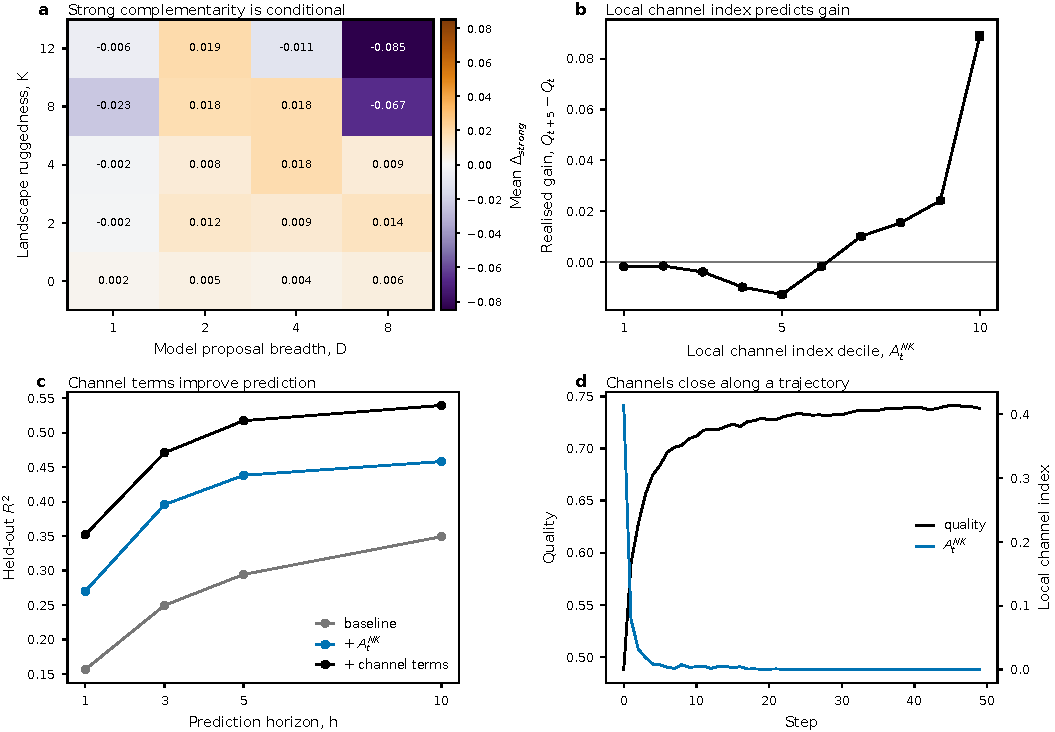
\includegraphics[width=0.97\linewidth]{figures/fig2_nk_local_channel.pdf}
\caption{\textbf{A local channel index predicts realised NK improvement.} \textbf{a}, Mean strong complementarity of the stabilised coupled system across landscape ruggedness and proposal breadth. \textbf{b}, Mean realised five-step gain by decile of the local NK channel index $\ANK_t$. \textbf{c}, Held-out prediction of future gain using a baseline model, the baseline plus $\ANK_t$, and the baseline plus additional channel terms. \textbf{d}, Mean quality and local channel index along stabilised coupled trajectories at $K=4,D=4$. The numerical values are parameter-dependent; the point is that a locally estimated channel quantity predicts future movement.}
\label{fig:nk_local_channel}
\end{figure}

\section*{Branching and agents}

The most direct empirical test is to branch conversations. Begin with a problem and an initial artefact $x_t$. Freeze the transcript and the artefact at a chosen turn. Then assign continuations to conditions: the same human alone, the model alone, the same human and model together, a new expert human, a new non-expert human, a relay chain or an agent population. The resulting artefacts are evaluated blind to condition.

This design separates the contributions of the original human, the model, the shared artefact and the coupling regime. If the intelligence resides mainly in the human, replacing the human should damage performance. If it resides mainly in the model, model-only continuations should preserve performance. If it resides in the coupled channel and shared artefact, a new competent human should be able to continue well from a well-structured state but not from a thin transcript.

The same design can estimate local operators. At a branch point, sample many possible next moves under controlled perturbations: different prompts, temperatures, role instructions, memory summaries or human framings. Code or embed the proposed moves in a common feature space. Their covariance estimates $J_t(C)$. Pairwise expert comparisons among nearby artefacts estimate $g_t$. Tests of whether combinations of local changes behave additively estimate curvature. These estimates allow a direct test of whether $g_t^\top J_tg_t$ predicts useful progress and whether $\tr[(J_t^{1/2}H_tJ_t^{1/2})^2]$ predicts failure or instability.

Agent systems extend the design from one human and one model to populations of human-like and model-like agents. Recent work shows that populations of large language model agents can form conventions and collective biases through local interactions \cite{Ashery2025}. The channel question is different: when do interacting agents create, preserve or corrupt epistemic channels? Three minimal tests are useful. In relay writing, each agent sees only the current artefact and contributes one move; the question is whether $\Aint_t$ decays or is preserved across handoffs. In critic--builder pairs, one agent proposes and another searches for curvature failures; the question is whether role partitioning reduces accepted harmful moves. In populations with memory, agents either inherit full transcripts or compressed state summaries; the question is whether state-like memory preserves channel alignment better than transcript-like memory.

A hierarchical model can estimate condition effects while accounting for task and participant variation:
\begin{equation}
    Q_{ijk} = \mu + \alpha_{C_i} + u_j + v_k + \epsilon_{ijk},
\end{equation}
where $C_i$ is the coupling condition, $u_j$ is a participant effect and $v_k$ is a task effect. The key posterior quantity is
\begin{equation}
    \Pr\{\DeltaStrong(\tau)>\delta \mid \text{data}\},
\end{equation}
where $\delta$ is a practically meaningful gain.

\section*{A restrained singularity}

The theory reframes the singularity question. A useful singularity concept should not begin with the claim that a machine becomes conscious. It should begin with a measurable transition in coupled cognitive systems. A coupled system crosses a threshold when it can sustain open-ended, self-correcting epistemic movement across tasks better than humans or models operating separately.

This threshold would not be determined by model size alone. It would depend on coupling bandwidth, memory, institutional feedback, expert evaluation, interface design, role partitioning and the structure of tasks. In this view, the singularity is less like a spark inside a machine and more like a change in the dynamics of a distributed system.

The consciousness question should remain separate. Performance evidence can show extended cognition, complementarity and perhaps global availability of information within a shared workspace. It cannot, by itself, establish phenomenal experience. The present theory therefore treats consciousness as a further question, not as a conclusion from the proposed experiments.

The practical message is to optimise channels, not merely answers. A good human--AI system should make the evaluative gradient clearer, generate variation in useful directions, expose curvature and preserve the right state of the artefact. This programme is testable now. It requires controlled tasks, branching histories, blinded evaluation and transparent logging of model versions and prompts. It also requires humility. Coupled systems will often fail. The point of the theory is not to praise human--AI collaboration, but to identify the conditions under which it becomes a real cognitive unit.

\section*{Methods}

\textbf{Local response derivation.} Let $P(u\mid x_t)$ be a zero-mean proposal distribution with covariance $J_t=\E[uu^\top\mid x_t]$. If proposals are developed with weight $w(u)=\exp(\eta g_t^\top u)$, then
\begin{equation}
    \E_w[u]=\frac{\E[u\exp(\eta g_t^\top u)]}{\E[\exp(\eta g_t^\top u)]}.
\end{equation}
Expanding numerator and denominator around $\eta=0$ gives $\E_w[u]=\eta J_tg_t+O(\eta^2)$. The same expansion with $Q(x_t+u)-Q(x_t)$ gives a linear contribution proportional to $g_t^\top J_tg_t$ plus higher-order terms governed by curvature and non-Gaussian proposal moments. Equation \ref{eq:interactional_channel_index} is a bounded diagnostic based on this separation.

\textbf{NK simulation.} NK landscapes used $N=16$, $K\in\{0,2,4,8,12\}$ and $D\in\{1,2,4,8\}$. For each $K$ we generated 32 random landscapes and starts. Each condition was run for 50 steps on the same landscape and start. Human-like proposals were mostly one-bit moves, with occasional two- and three-bit moves. Model-like proposals had maximum Hamming distance $D$ and were sampled with probability increasing with distance. The human-like evaluator had lower noise than the model-like evaluator; uncertainty increased with $K$ and proposal distance. The stabilised coupled condition accepted a move only when its estimated gain exceeded $0.70$ evaluator standard deviations.

\textbf{Local channel analysis.} Along stabilised coupled trajectories, we sampled 96 proposals per state from the same proposal distribution. For each proposal we computed the true quality change, the local additive prediction from single-bit effects, the nonlinear residual, evaluator uncertainty, the local channel index $\ANK_t$, the channel potential, misleading-proposal fraction and curvature liability. Future realised gains were $Q_{t+h}-Q_t$ for $h\in\{1,3,5,10\}$.

\textbf{Prediction models.} Prediction models were ordinary least squares models trained and tested on held-out landscapes. The baseline used current quality, step, $K$ and $D$. The index model added $\ANK_t$. The channel model added $\ANK_t$, channel potential, misleading-proposal fraction and curvature liability. Predictors were centred and scaled using the training set. Reported $R^2$ values are out-of-sample values on held-out landscapes.

\textbf{Robustness checks.} Sensitivity checks used smaller runs to vary stabilisation margin, state size and model proposal number. These checks are not exhaustive. They test whether the local-channel prediction survives reasonable perturbations of the illustrative model.

\textbf{Data and code availability.} The present draft package contains all code, random seeds, generated CSV files and figure scripts needed to reproduce the illustrative simulations and figures. A public repository and archived release will be prepared before submission.

\textbf{AI-use disclosure.} A large language model was used as a drafting, coding and structuring aid for this manuscript version. Final responsibility for claims, citations, analysis, wording and submission rests with the human authors. The model is not an author.

\section*{Acknowledgements}

To be completed. This draft grew from discussions about additive genetic channels, epistemic landscapes, human--AI complementarity and the mathematical habits needed to make such analogies testable.

\section*{Funding}

To be completed.

\section*{Author contributions}

To be completed.

\section*{Competing interests}

To be completed.

\section*{Extended Data legends}

\textbf{Extended Data Fig. 1 | Descriptive NK outcomes.} \textbf{a}, Final quality across landscape ruggedness at $D=4$. \textbf{b}, Mean search trajectories on an intermediate landscape. \textbf{c}, Mean strong complementarity of the stabilised coupled system across proposal breadth and ruggedness. \textbf{d}, Fraction of accepted moves that lower true quality under broad proposals. These panels show the descriptive behaviour behind Fig. \ref{fig:nk_local_channel}.

\textbf{Extended Data Fig. 2 | Sensitivity of local-channel prediction.} Gain in held-out $R^2$ at horizon $h=5$ after adding the local channel index or fuller channel terms to the baseline model. The checks vary stabilisation margin, state size and model proposal number.

\clearpage
\begin{thebibliography}{99}

\bibitem{Clark1998}
Clark, A. \& Chalmers, D. The extended mind. \textit{Analysis} \textbf{58}, 7--19 (1998).

\bibitem{Hutchins1995}
Hutchins, E. \textit{Cognition in the Wild}. MIT Press (1995).

\bibitem{Hollan2000}
Hollan, J., Hutchins, E. \& Kirsh, D. Distributed cognition: toward a new foundation for human-computer interaction research. \textit{ACM Transactions on Computer-Human Interaction} \textbf{7}, 174--196 (2000).

\bibitem{Vaccaro2024}
Vaccaro, M., Almaatouq, A. \& Malone, T. When combinations of humans and AI are useful: a systematic review and meta-analysis. \textit{Nature Human Behaviour} \textbf{8}, 2293--2303 (2024).

\bibitem{Gonzalez2026}
Gonzalez, C. et al. Toward a science of human--AI teaming for decision making: a complementarity framework. \textit{PNAS Nexus} \textbf{5}, pgag030 (2026).

\bibitem{DellAcqua2026}
Dell'Acqua, F. et al. Navigating the jagged technological frontier: field experimental evidence of the effects of AI on knowledge worker productivity and quality. \textit{Organization Science} (2026). doi:10.1287/orsc.2025.21838.

\bibitem{Wright1932}
Wright, S. The roles of mutation, inbreeding, crossbreeding and selection in evolution. \textit{Proceedings of the Sixth International Congress of Genetics} \textbf{1}, 356--366 (1932).

\bibitem{Lande1979}
Lande, R. Quantitative genetic analysis of multivariate evolution, applied to brain:body size allometry. \textit{Evolution} \textbf{33}, 402--416 (1979).

\bibitem{LandeArnold1983}
Lande, R. \& Arnold, S. J. The measurement of selection on correlated characters. \textit{Evolution} \textbf{37}, 1210--1226 (1983).

\bibitem{Kauffman1987}
Kauffman, S. A. \& Levin, S. Towards a general theory of adaptive walks on rugged landscapes. \textit{Journal of Theoretical Biology} \textbf{128}, 11--45 (1987).

\bibitem{Weinberger1991}
Weinberger, E. D. Local properties of Kauffman's N-k model: a tunably rugged energy landscape. \textit{Physical Review A} \textbf{44}, 6399--6413 (1991).

\bibitem{NowakMay1992}
Nowak, M. A. \& May, R. M. Evolutionary games and spatial chaos. \textit{Nature} \textbf{359}, 826--829 (1992).

\bibitem{Nowak2004Nature}
Nowak, M. A., Sasaki, A., Taylor, C. \& Fudenberg, D. Emergence of cooperation and evolutionary stability in finite populations. \textit{Nature} \textbf{428}, 646--650 (2004).

\bibitem{NowakSigmund2004}
Nowak, M. A. \& Sigmund, K. Evolutionary dynamics of biological games. \textit{Science} \textbf{303}, 793--799 (2004).

\bibitem{Nowak2006}
Nowak, M. A. Five rules for the evolution of cooperation. \textit{Science} \textbf{314}, 1560--1563 (2006).

\bibitem{Ohtsuki2006}
Ohtsuki, H., Hauert, C., Lieberman, E. \& Nowak, M. A. A simple rule for the evolution of cooperation on graphs and social networks. \textit{Nature} \textbf{441}, 502--505 (2006).

\bibitem{Ashery2025}
Flint Ashery, A., Aiello, L. M. \& Baronchelli, A. Emergent social conventions and collective bias in LLM populations. \textit{Science Advances} \textbf{11}, eadu9368 (2025).

\end{thebibliography}

\clearpage
\begin{figure}[p]
\centering
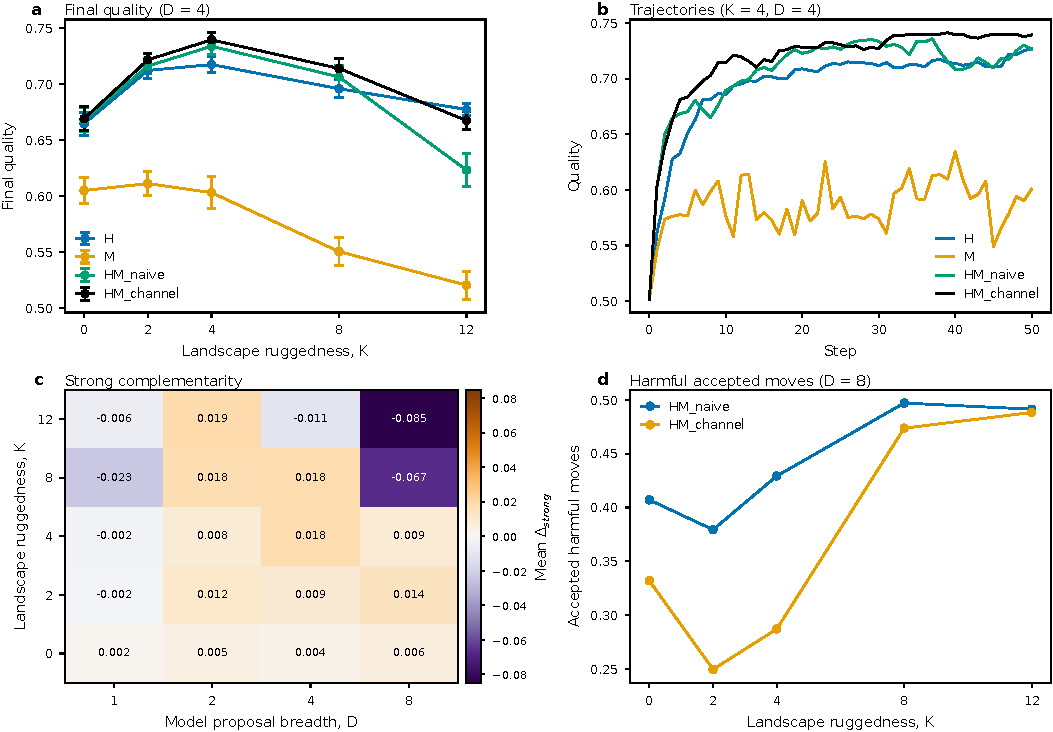
\includegraphics[width=0.97\linewidth]{extended_data/extended_data_fig1_nk_summary.pdf}
\caption*{\textbf{Extended Data Fig. 1 | Descriptive NK outcomes.} Panels show final quality, search trajectories, strong complementarity and harmful accepted moves in the illustrative NK model.}
\end{figure}

\begin{figure}[p]
\centering
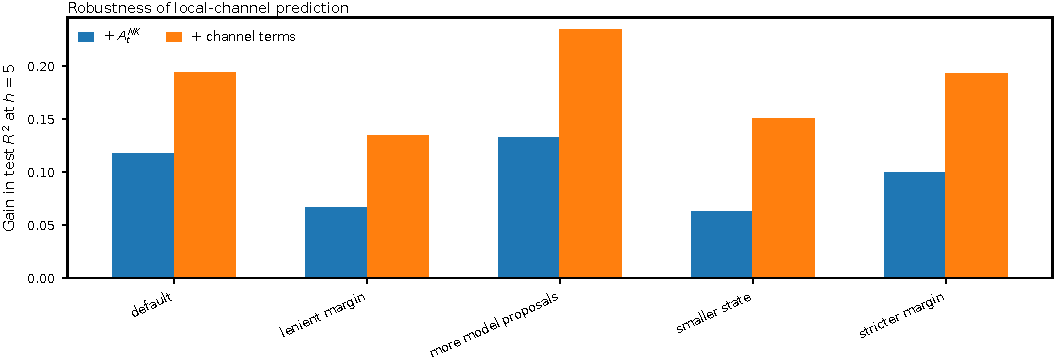
\includegraphics[width=0.97\linewidth]{extended_data/extended_data_fig_robustness.pdf}
\caption*{\textbf{Extended Data Fig. 2 | Sensitivity of local-channel prediction.} Gain in held-out $R^2$ at horizon $h=5$ under small parameter perturbations.}
\end{figure}

\end{document}
